\chapter{Experimental Results}
\label{chapter6_experiments}
\thispagestyle{empty}

\vspace{0.5cm}

In this chapter we show experimental results of our algorithm on some Atari
games.
We show that the representation of the states learned by our feature extraction 
pipeline is suitable for the semi-batch control approach with FQI, and that 
our agent is able to learn non-trivial policies with good sample efficiency on 
different environments.

\section{Premise}
Our approach aims at optimizing sample efficiency, but does not account for
the computational complexity of training and evaluating the full pipeline. 
All three main components of the algorithm benefit a great deal from parallel 
computing, to the point where the hardware itself is a key component in 
making the algorithm treatable at all. 
We were thus strongly limited in our experimental phase by our access to 
hardware for heavy parallel computing, with even costs for renting servers on 
cloud providers being prohibitive when considering our runtime. 
We therefore had to be extremely selective in what experiments to run, each of 
which took days at a time, and well balanced between exploring new possibilities
(hyperparameters, network architectures, environments) and evaluating current 
configurations. 
In this chapter we report the best findings across all our experiments and we 
try to outline the thought process that led us to favor some choices over others.
The hardware configurations of the three servers that we used for experiments is
reported in Table \ref{t:servers}. 
%
\begin{table}[t]
    \centering
    \begin{tabular}{c c c c} 
	\hline
	Server ID & vCPU count & GPU                          & RAM (GB) \\ 
	\hline 
	\#$1$     & $64$       & None                         & $252$ \\
	\#$2$     & $8$        & $1 \times$ Nvidia Tesla K40C & $32$ \\
	\#$3$     & $4$        & $1 \times$ Nvidia Tesla K40C & $32$ \\
	\hline
    \end{tabular}
    \caption[Server configurations for experiments]{Server configurations for 
	     experiments.}
    \label{t:servers}
\end{table}
%

The code implementation of the algorithm was based on Python 2.7 and its 
\textit{de facto} standard libraries for general machine learning, GPU-based 
deep learning, and linear algebra. 
We trained and used the AE on an \textit{Nvidia Tesla K40C} GPU, using the 
\textit{Keras 2.0.6} API as interface to the \textit{Tensorflow 1.3.0} library 
for deep learning, whereas the training and evaluation of Extra-Trees 
for RFS and FQI was run on CPU using the \textit{Scikit-Learn 0.19.0} library.
We used the implementations of FQI and RFS provided in the open source 
\textit{IFQI} library by Matteo Pirotta.
Finally data manipulation and any other algebraic operations were done with 
\textit{Numpy 1.13.1}.

\section{Baseline}\label{s:exp_baseline}
To evaluate the results of our approach with respect to other algorithms, we 
compared our agent's performance with that of DQN \cite{mnih2015human} and of a 
fully random policy. 
For DQN, we used an open source implementation of the paper by Mnih et al.\  
with the same exact parametrization, and run the algorithm for a total of $50$ 
million online training samples on the \textit{Breakout, Pong}, and 
\textit{Space Invaders} environments from the Atari games.
To remain loyal to the original DQN methodology, we run an evaluation phase 
of $125000$ steps every $250000$ collected training samples, and we considered
the average cumulative non-clipped reward across the episodes completed in
this period. A similar evaluation was also run once on the fully random policy.
The best performance achieved by the baseline algorithms is reported in Table 
\ref{t:envs_used} and we show the learning curve of DQN across the $50$ million
frames in Figures \ref{f:BO_baseline}, \ref{f:P_baseline} and \ref{f:SI_baseline}.
%
\begin{table}[b]
    \centering
    \begin{tabular}{l c c c c} 
	\hline
	Environment    & $|A|$ & Random   & Best DQN  & Samples for best DQN \\ 
	\hline 
	Breakout       & $4$   & $1.09$   & $319.83$  & $\approx19250000$ \\
	Pong           & $6$   & $-20.49$ & $19.82$   & $\approx35250000$ \\
	Space Invaders & $6$   & $174.46$ & $1125.41$ & $\approx31500000$ \\
	\hline
    \end{tabular}
    \caption[Performance of baseline algorithms]{Average performance of baseline
	     algorithms.}
    \label{t:envs_used}
\end{table}
%
%
\begin{figure}
    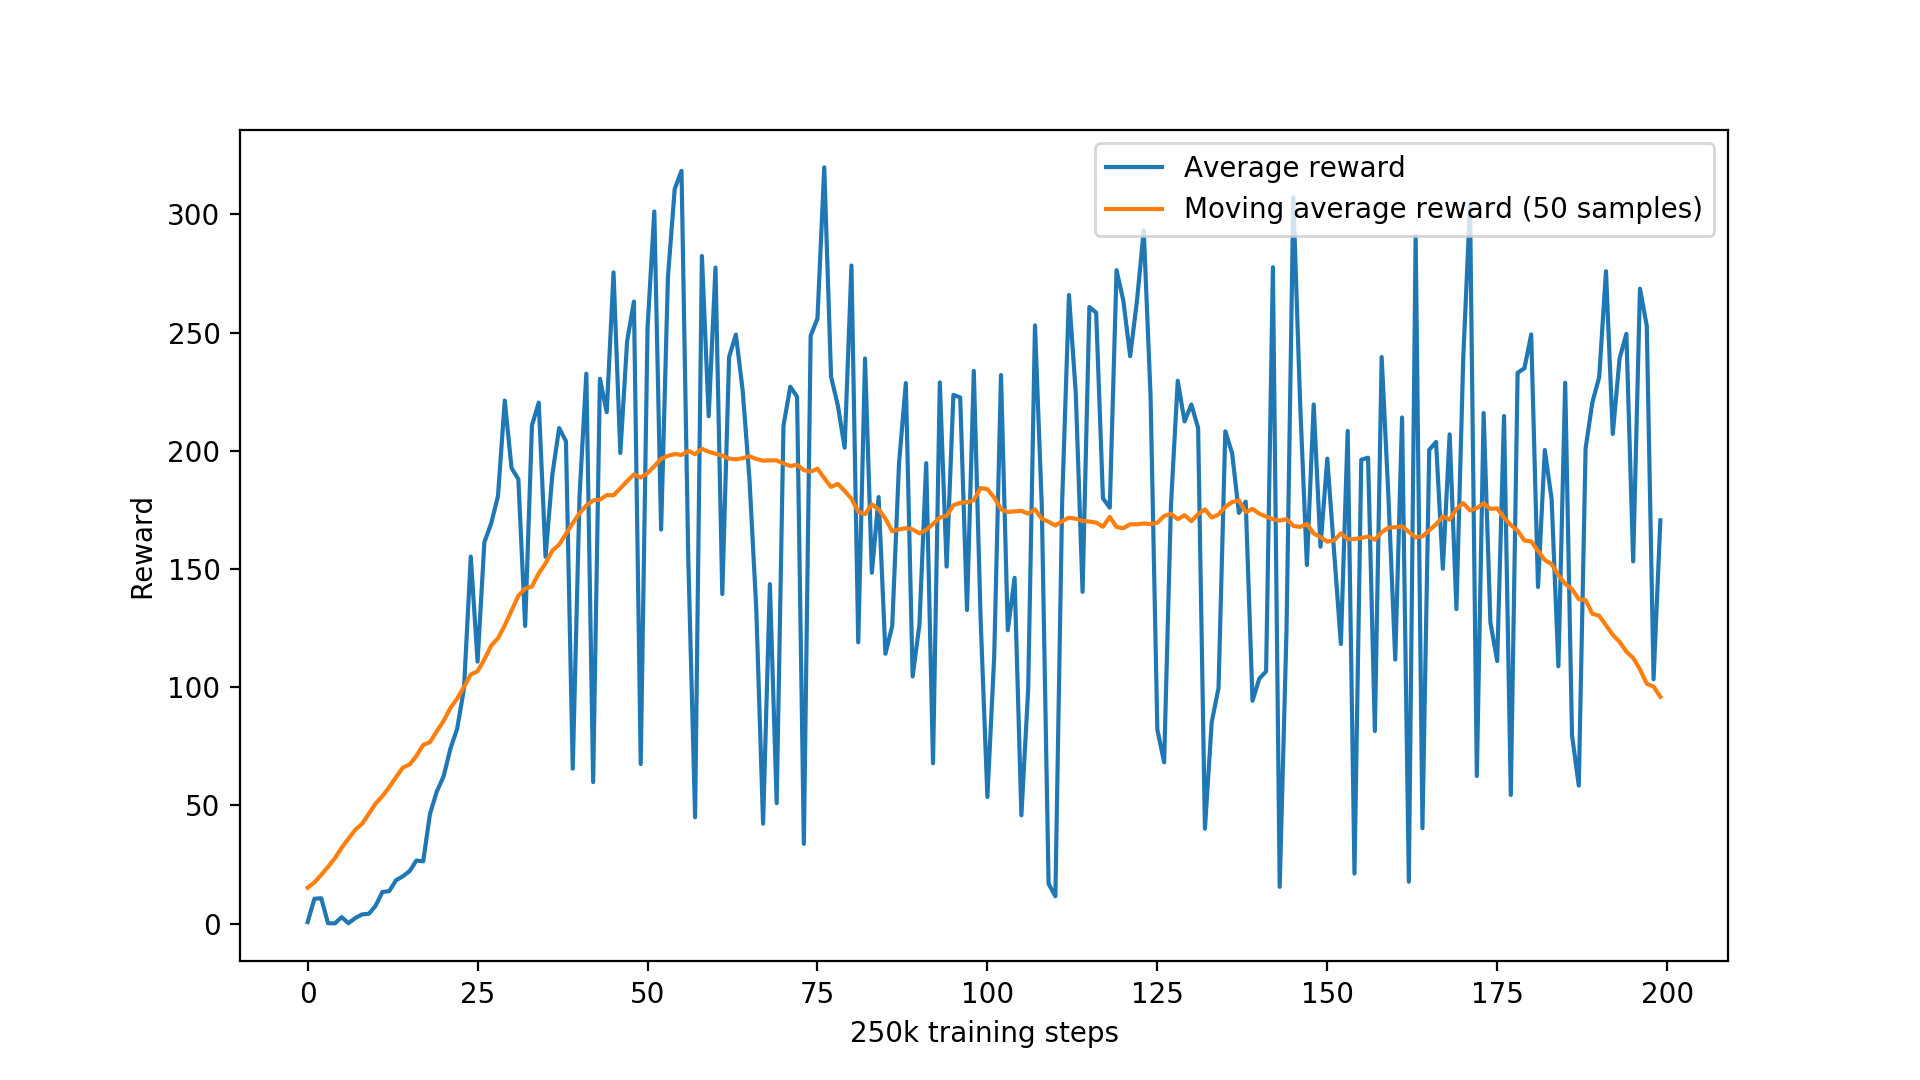
\includegraphics[width=\textwidth]{pictures/experiments/baseline_breakout}
    \centering
    \caption[Average performance of DQN in Breakout]{Average evaluation reward 
	    of DQN in Breakout (each point is the average score over $125000$
	    evaluation steps).}
    \label{f:BO_baseline}
\end{figure}
%
%
\begin{figure}
    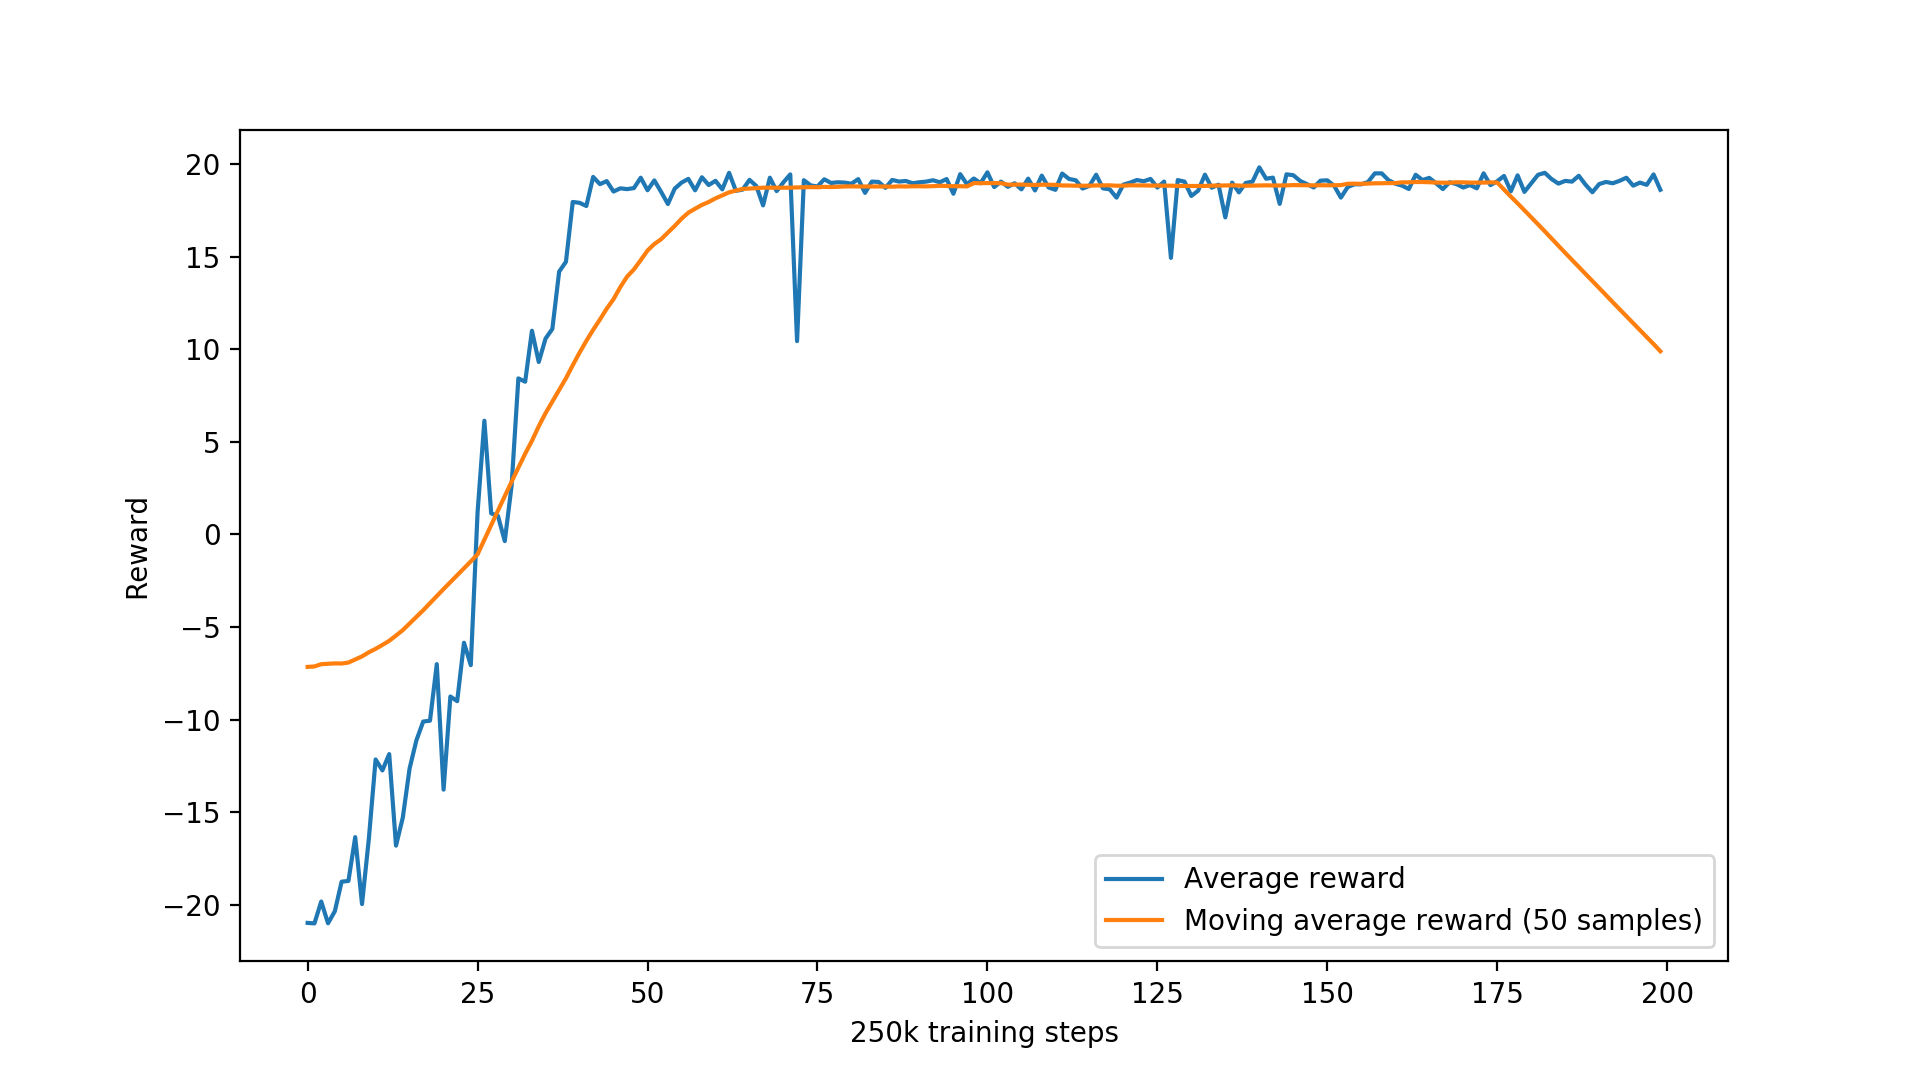
\includegraphics[width=\textwidth]{pictures/experiments/baseline_pong}
    \centering
    \caption[Average performance of DQN in Pong]{Average evaluation reward 
	    of DQN in Pong (each point is the average score over $125000$
	    evaluation steps).}
    \label{f:P_baseline}
\end{figure}
%
%
\begin{figure}
    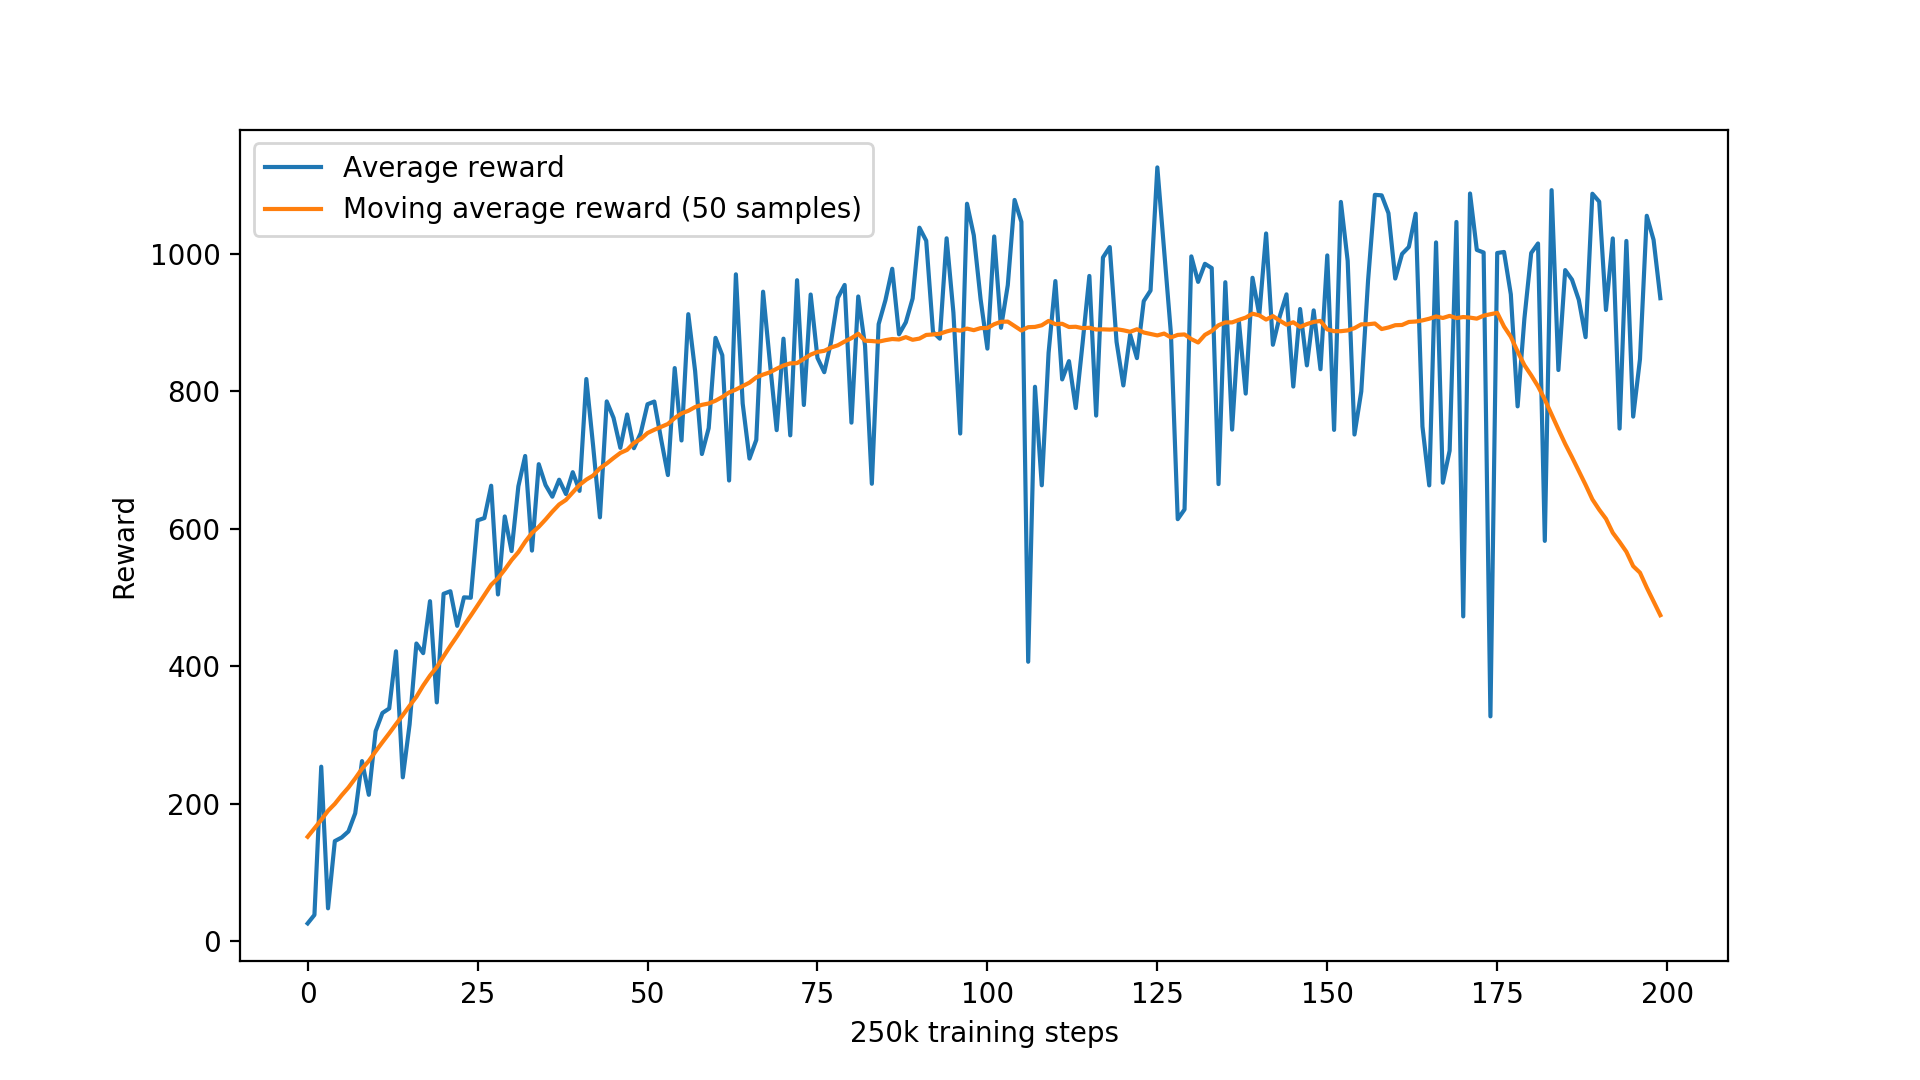
\includegraphics[width=\textwidth]{pictures/experiments/baseline_space_invaders}
    \centering
    \caption[Average performance of DQN in Space Invaders]{Average evaluation reward 
	    of DQN in Space Invaders (each point is the average score over $125000$
	    evaluation steps).}
    \label{f:SI_baseline}
\end{figure}
%

\section{Autoencoder}
Due to the extremely high training and (especially) evaluation times that we 
encountered in FQI\footnote{Slow performance in evaluation is due to the 
sample-wise forward prediction across the full pipeline required at each step
of evaluation episodes. Specifically, each prediction of the $Q$ function needs 
a forward pass of the 4-layer encoder (which requires loading data in the GPU)
and a forward pass of Extra-Trees (which due to an internal inefficiency in 
\textit{Scikit-learn} was extremely slow when predicting on a single sample).},
and the almost intractable runtime of RFS\footnote{Which can take more than a 
week to complete, on our most performing server.}, we had to formally assess the 
suitability of the extracted features for control problems before moving on to 
training the other components in the pipeline. 
To do so, we run a series of tests devised to highlight different aspects of
success in the feature extraction. Once a training configuration was deemed 
satisfactory, we kept it fixed for all the following experiments.
%
\begin{table}
    \centering
    \begin{tabular}{l c c c} 
	\hline
	Environment                     & $\varepsilon$ & Val. loss        & Val. accuracy \\ 
	\hline 
	\multirow{3}{*}{Breakout}       & $1.0$         & $\approx10^{-5}$ & $1.0$    \\
	                                & $0.55$        & $\approx10^{-4}$ & $0.9999$ \\
	                                & $0.1$         & $\approx10^{-4}$ & $0.9997$ \\
	\hline
	\multirow{3}{*}{Pong}           & $1.0$         & $\approx10^{-4}$ & $0.9999$ \\ 
	                                & $0.55$        & $\approx10^{-4}$ & $0.9997$ \\
	                                & $0.1$         & $\approx10^{-4}$ & $0.9993$    \\
	\hline
	\multirow{3}{*}{Space Invaders} & $1.0$         & $\approx10^{-3}$ & $0.9987$ \\
	                                & $0.55$        & $\approx10^{-3}$ & $0.9985$ \\
	                                & $0.1$         & $\approx10^{-3}$ & $0.9978$ \\
	\hline
    \end{tabular}
    \caption[AE validation performance]{Validation performance of our AE on
	     fully random datasets of $\approx50000$ samples.}
    \label{t:ae_training_precision}
\end{table}
%
%
\begin{figure}
    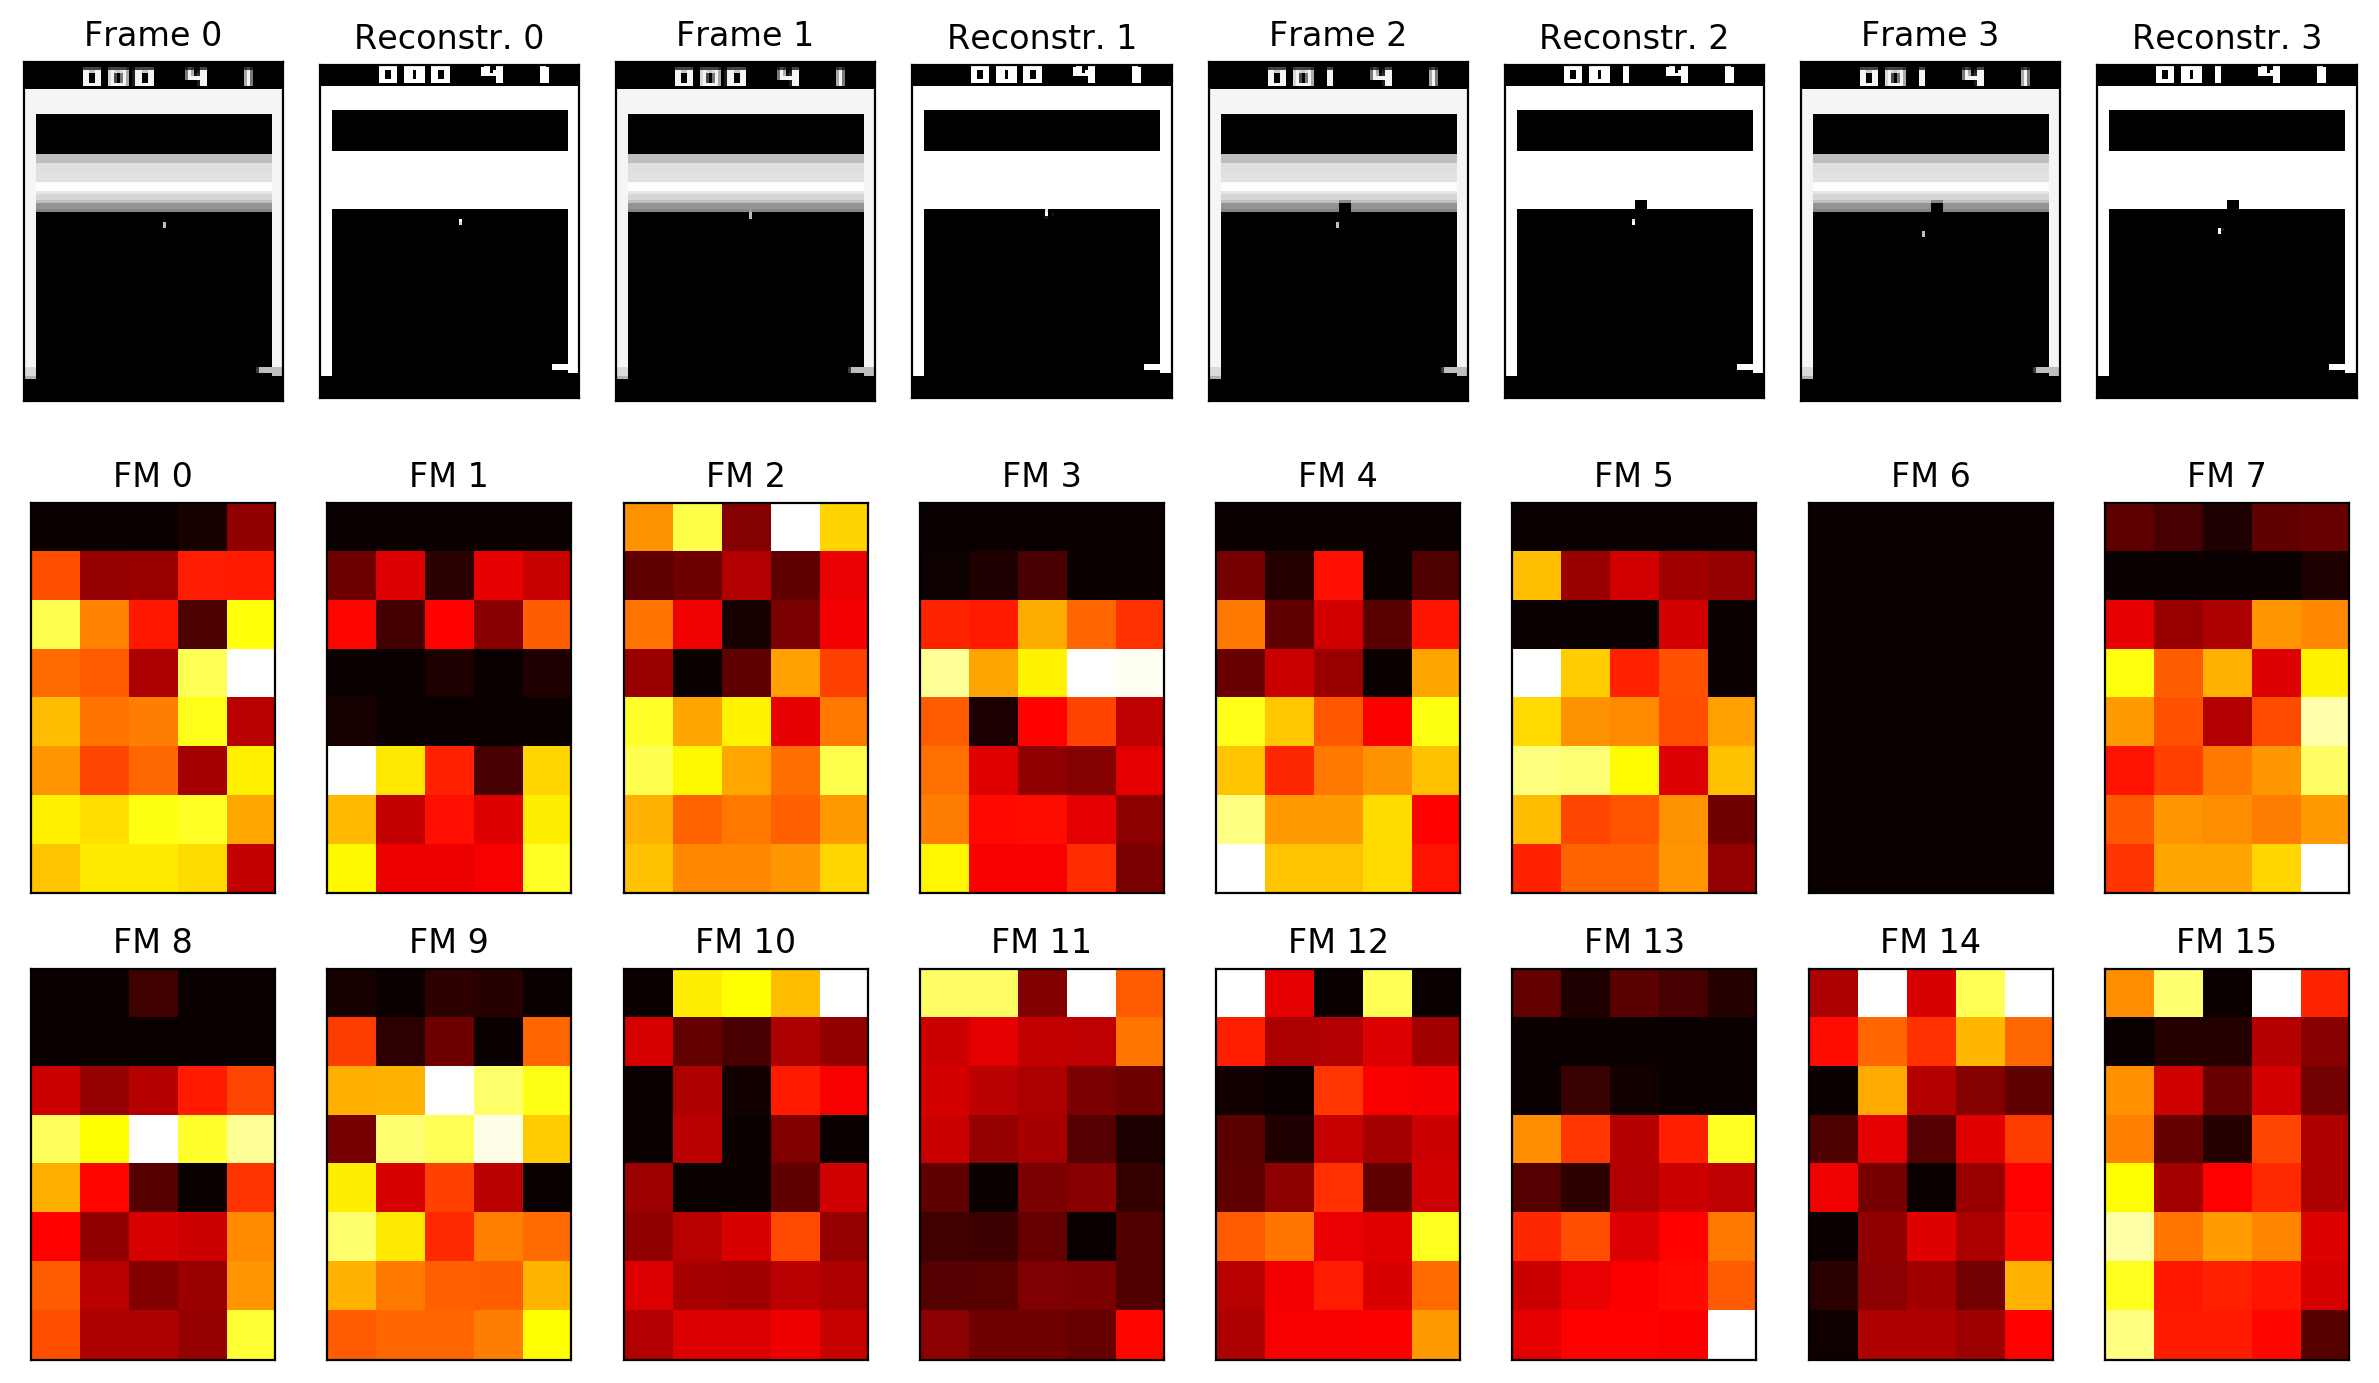
\includegraphics[width=\textwidth]{pictures/experiments/reconstr_breakout}
    \centering
    \caption[AE reconstruction and feature maps on Breakout]{AE reconstruction 
	    and feature maps on Breakout. 
	    Each pair in the top row shows a frame of a $4$-channel state $s$ 
	    given as input to the AE, with its associated reconstructed channel. 
	    The bottom two rows show the relative activation values of the 
	    innermost feature maps before the flatten layer, after encoding $s$: 
	    colors represent a \textit{heatmap} from black ($0$) to white 
	    (map-wise maximum activation value). The same applies to Figures 
	    \ref{f:P_reconstr} and \ref{f:BO_reconstr}.}
    \label{f:BO_reconstr}
\end{figure}
%
%
\begin{figure}
    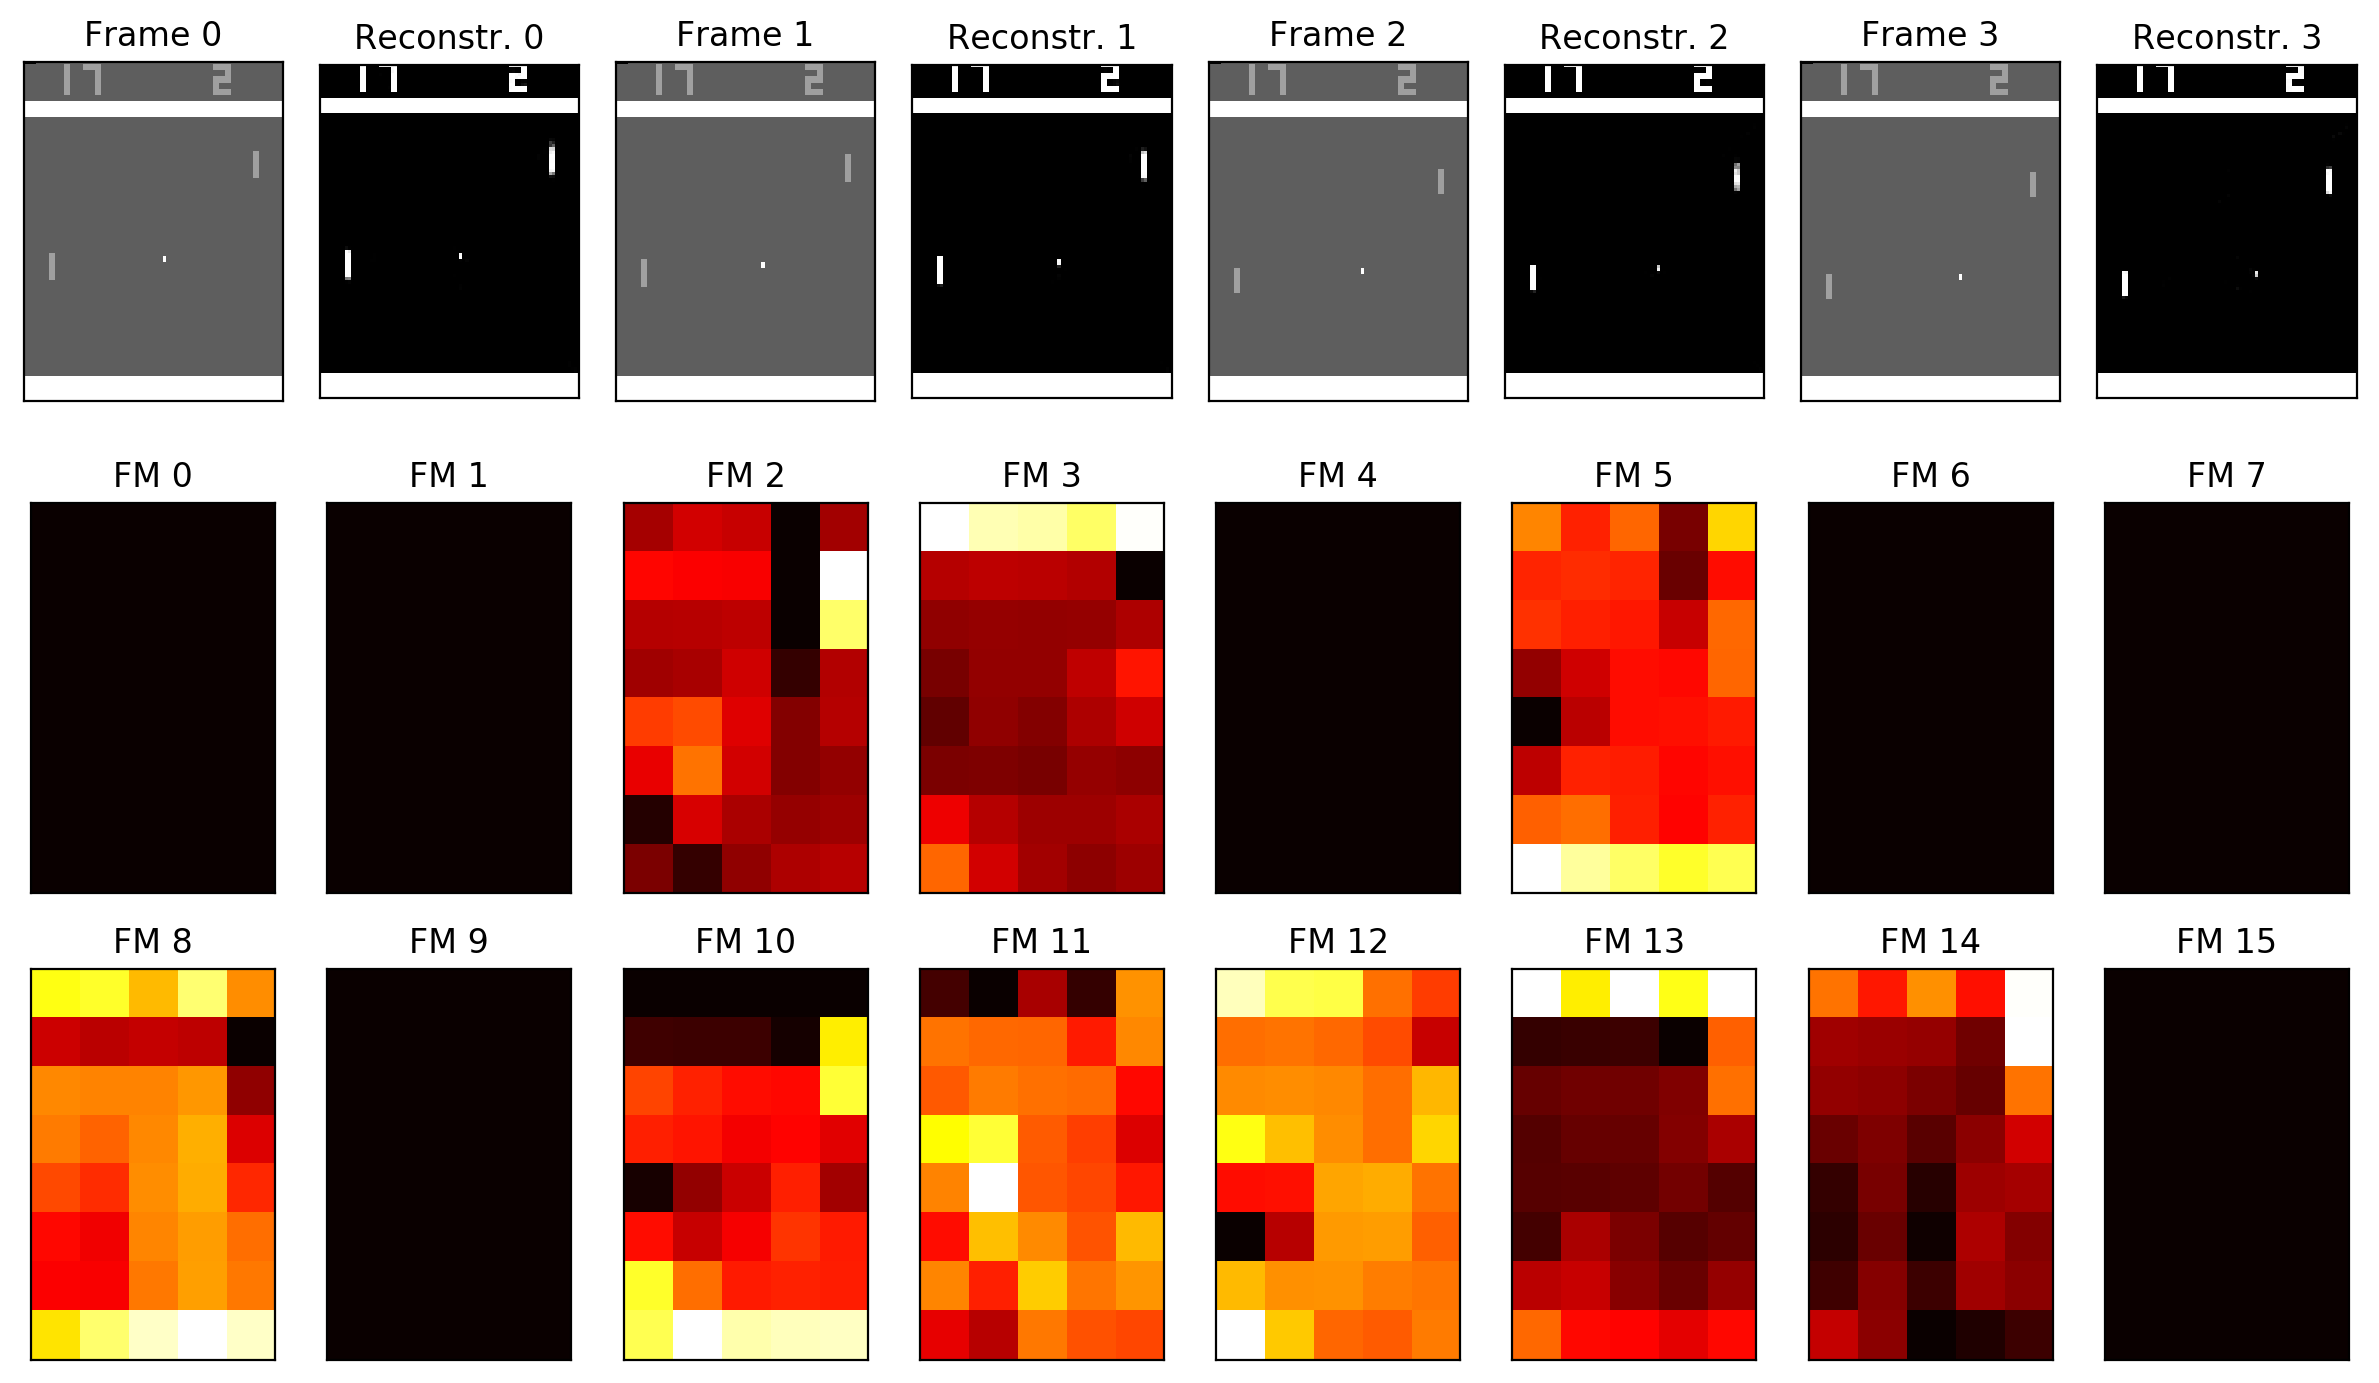
\includegraphics[width=\textwidth]{pictures/experiments/reconstr_pong}
    \centering
    \caption[AE reconstruction and feature maps on Pong]{AE reconstruction 
	    and feature maps on Pong.}
    \label{f:P_reconstr}
\end{figure}
%
%
\begin{figure}
    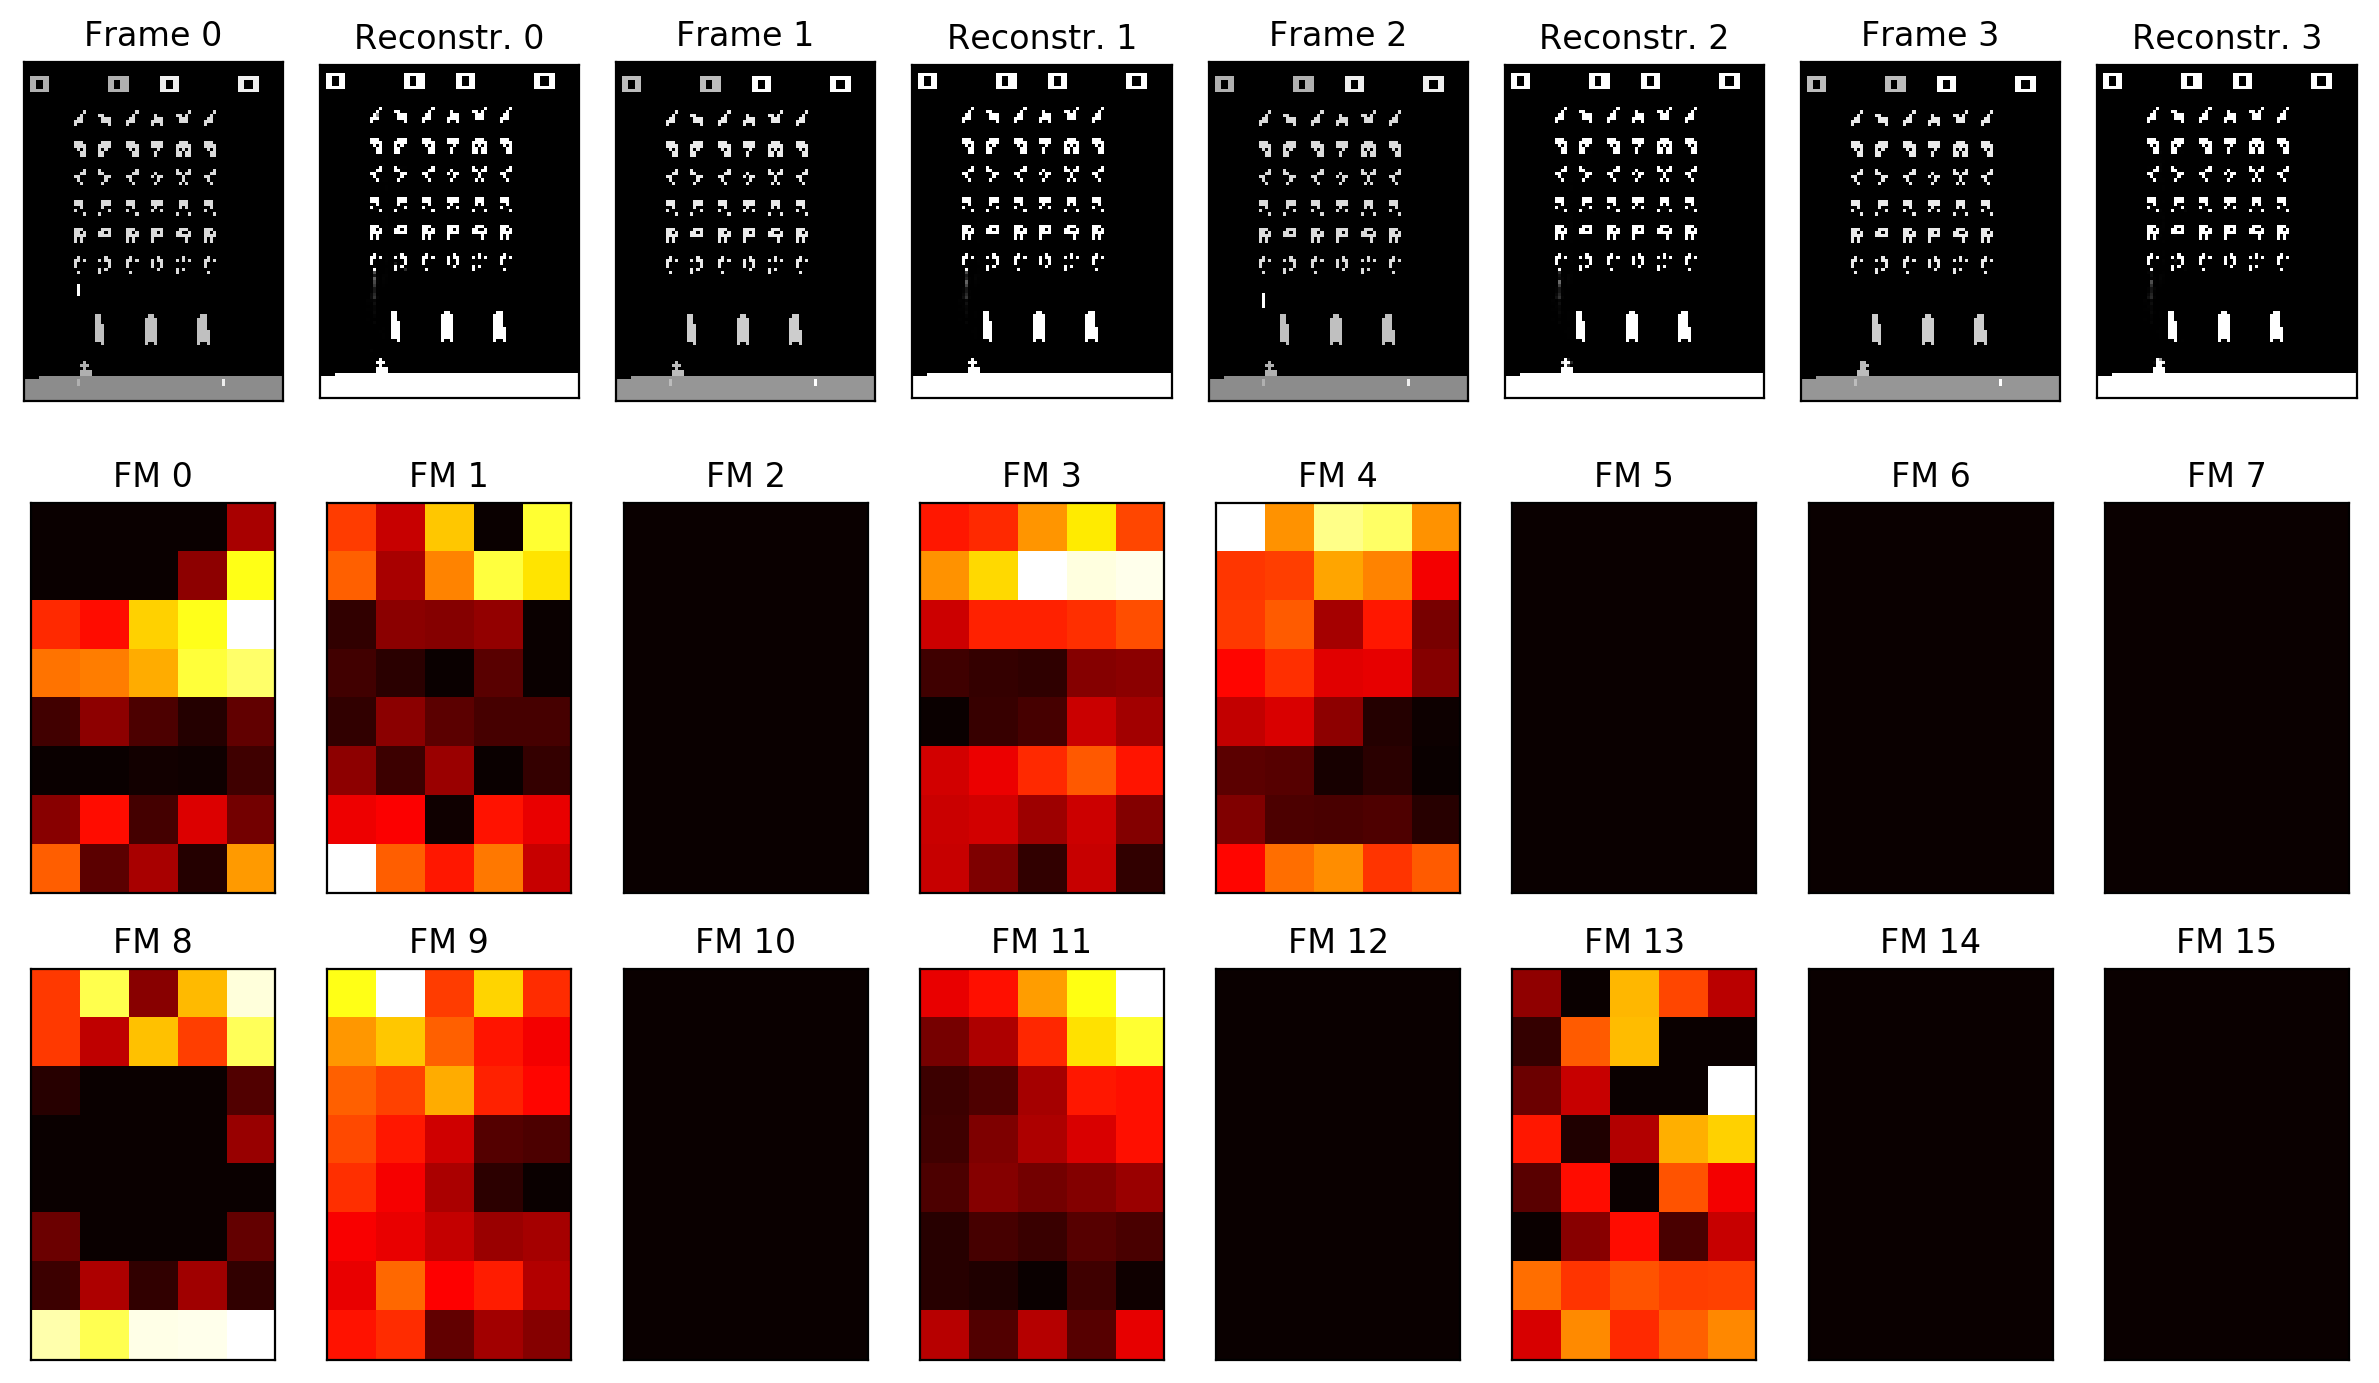
\includegraphics[width=\textwidth]{pictures/experiments/reconstr_space_invaders}
    \centering
    \caption[AE reconstruction and feature maps on Space Invaders]{AE 
	    reconstruction and feature maps on Space Invaders. Note that the 
	    lower accuracy here translates to a poor definition in 
	    reconstructing moving elements like the player's character and 
	    projectiles.}
    \label{f:SI_reconstr}
\end{figure}
%

The most simple test that we run consisted in assessing the reconstruction loss
and accuracy of the AE on a held-out validation set (cf.\ Section \ref{s:ae_training_details}). 
We were able to achieve very high reconstruction accuracy in all environments, 
with no sensible differences between training sets collected under different 
exploration rates. In Table \ref{t:ae_training_precision} we report validation 
performance of the AE on datasets of $\approx50000$ samples collected with 
different values of $\varepsilon$ (see also Figures \ref{f:BO_reconstr}, 
\ref{f:P_reconstr}, and \ref{f:SI_reconstr}). 
In general, the reconstruction of the AE is better when the training dataset is
collected under a high exploration rate. This is intuitively due to the fact 
that more random policies are less effective and can only reach a few states, so
that the AE has to learn a simpler representation of the environment (e.g.\ 
there is no point in learning to reconstruct the higher layers of the wall in 
Breakout if the agent never breaks them).
This does not apply to environments like Pong in which the agent has no effect 
on the fixed elements of the game, and for which we see an almost constant
reconstruction accuracy with all exploration rates. 
Less formally, a visual inspection of the reconstruction helped us in the early 
experimental phases and highlighted how even a small change in accuracy (in the
order of $10^{-3}$) could result in an incredibly noisy output. This can be
seen in Figure \ref{f:SI_reconstr}, where a $99.8\%$ reconstruction accuracy 
on Space Invaders means that the AE is not able to reconstruct some small moving 
elements of the game.

At the same time, we also inspected the values and behaviors of the features 
maps produced by the encoder before flattening, by creating short animations 
(See Figures \ref{f:BO_reconstr}, \ref{f:P_reconstr}, and \ref{f:SI_reconstr}) 
of how the activation values changed in a sequence of about a hundred states. 
This confirmed that the extracted features maps contained abstract enough 
information (without excessive spatial correlation between the features). We 
also observed that in Space Invaders, on average, almost half of the features
\textit{died}. This phenomenon is a common occurrence in CNNs that use the ReLU 
activation function (due to the fact that ReLU has a null gradient for
all inputs lower or equal than zero, cf.\ Figure \ref{f:relu_sigmoid}), but
we were not able to explain such a high death rate on this particular 
environment, which presents a more complicated structure than the other
environments that we tested.
%
\begin{table}[t]
    \centering
    \begin{tabular}{l c c c} 
	\hline
	Environment                     & $\varepsilon$ & $R^2$   & MSE \\ 
	\hline 
	\multirow{3}{*}{Breakout}       & $1.0$         & $0.937$ & $0.0272$ \\
	                                & $0.55$        & $0.854$ & $0.0761$ \\
	                                & $0.1$         & $0.855$ & $0.0748$ \\
	\hline
	\multirow{3}{*}{Pong}           & $1.0$         & $0.945$ & $0.0167$ \\
	                                & $0.55$        & $0.849$ & $0.0334$ \\
	                                & $0.1$         & $0.905$ & $0.0241$ \\
	\hline
	\multirow{3}{*}{Space Invaders} & $1.0$         & $0.532$ & $0.3895$ \\
	                                & $0.55$        & $0.468$ & $0.5032$ \\
	                                & $0.1$         & $0.457$ & $0.5126$ \\
	\hline
    \end{tabular}
    \caption[Results of $\tilde{S}$-$Q$ mapping experiment]{Results of the 
	     $\tilde{S}$-$Q$ mapping experiment with different exploration rates
	     to collect the datasets.}
    \label{t:FQ_tests}
\end{table}
%

In order to truly assess the compatibility of the extracted features 
with control problems, we also trained a supervised model to learn the $Q$ 
approximation produced by DQN using the extracted features (we call this 
an \textit{$\tilde{S}$-$Q$ test}). 
We used a training set composed of tuples $(ENC(s) \in \tilde{S}, q \in \mathbb{R}^{|A|})$, 
where $s$ is a state from the environment, after the preprocessing described in 
Section \ref{s:atari_envs}, and $q$ is the $|A|$-dimensional estimate produced 
by DQN when it receives $s$ as input. 
Note that we could use the same input for both networks, because the 
preprocessing that we perform on the observations before feeding a sample to the
encoder (cf.\ Section \ref{s:atari_envs}) is basically the same that is 
applied to the inputs for DQN. To account for the slight different preprocessing,
we computed $q$ before applying the transformations which are unique to our 
preprocessing, namely the binarization and cropping. 
For each environment, we used the best performing DQN (as per Section \ref{s:exp_baseline}) 
to produce the targets, and we sampled $\approx50000$ states from the same 
dataset on which the AE was trained.
To learn the $Q$ approximation, we used the same Extra-Trees model and 
hyperparameters that we use for FQI (See Table \ref{t:FQI_tree_params}), to 
ensure that the configuration itself was adequate to describe the nonlinear 
relations between the features and the action-value function at convergence of 
FQI. 
This was done by simply fitting the model on the $(ENC(s), q)$ pairs, and 
evaluating the $R^2$ score (cf.\ Definition \eqref{e:R2}) and \textit{Mean 
Squared Error} (MSE) of the predictions on a held-out validation set of roughly 
$5\%$ of the training samples.
As seen in Figure \ref{f:FQ_test_all_three}, the extracted features are suitable
for describing the $Q$ function learned by DQN with a good degree of precision, 
and constitute an adequate base for our whole approach. 
We are able to obtain an average $R^2$ score of $0.88$, $0,90$, and $0.48$ on 
all three tested environments respectively.
Similarly to what we observed for the AE, in Space Invaders we have a drop in 
performance probably due to a difficulty in representing all elements in 
the environment. For instance, since the AE is not able to properly represent 
the character and its projectiles, we can assume that there are no features that
describe these elements. However, these are essential to predict the reward 
and, consequently, the $Q$ function, and their absence could explain the bad
prediction.
We report the results of these tests, run on datasets collected with different
values of $\varepsilon$ at different iterations of our full algorithm, in 
Table \ref{t:FQ_tests}.
%
\begin{figure}
    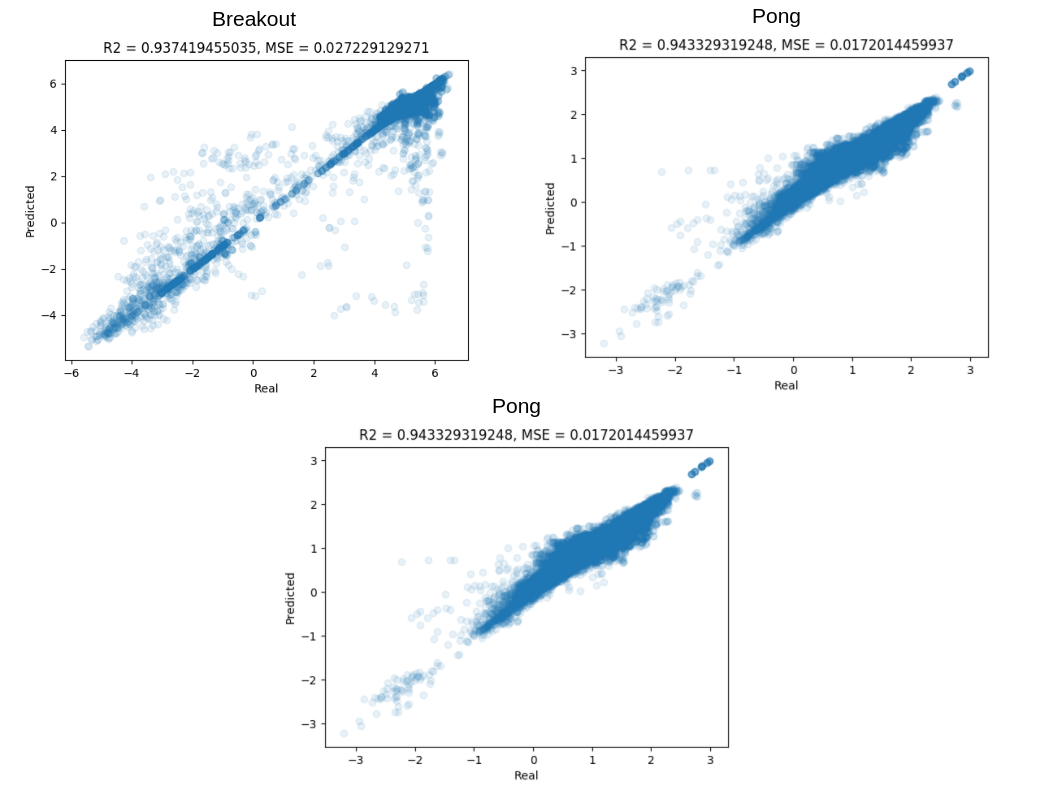
\includegraphics[width=\textwidth]{pictures/experiments/FQ_test_all_three}
    \centering
    \caption[Predictions of $\tilde{S}$-$Q$ mapping experiment]{Values predicted 
	     by the supervised model in the $\tilde{S}$-$Q$ test vs.\ real 
	     values predicted by DQN. Note that the $|A|$-dimensional estimate 
	     of the $Q$ function is flattened and treated as a sequence of 
	     $|A|$ independent values in order to plot it.}
    \label{f:FQ_test_all_three}
\end{figure}
%

\section{Recursive Feature Selection}
The main purpose of RFS in our learning pipeline is to provide a fast forward 
propagation of the AE at control time, by keeping only the AE weights that are 
essential for the representation. 
The runtime of RFS, however, is the longest amongst the three main components, 
taking up to a week to complete and extending the runtime of the full algorithm
to a point where it becomes unfeasible. We therefore had to ignore RFS 
during most of our experiments, resorting to only running it once per 
environment using a dataset collected under a fully random policy and an AE 
trained on the same dataset (as if we were running the selection at the first 
step of the main procedure). 
At the same time, we found it appropriate to run another simple feature 
selection technique which consisted in only keeping those features with nonzero 
variance (NZV), in order to simplify our feature space without losing 
information. 
We found that RFS reduced the representation by up to $60\%$ with respect to NZV
on Pong, which indicates that the AE does indeed extract a great deal of 
redundancy that can be ignored for control purposes. 
However, we were not able to replicate this performance on the other two 
environments.
In Breakout, RFS only selected four state features and did not select the action. 
On the other hand, this behavior was inverted on Space Invaders, where the 
procedure selected all state and action features (including those with zero 
variance removed by NZV) at the first step, when explaining the reward. 
The reason for this inconsistent behavior by RFS is probably due to an 
incompatibility between the RFS procedure itself and the dynamics of the 
features extracted by the AE but, as we will show in the following sections,
this does not prevent the agent from learning a good policy using the 
AE's representation.
In Figures \ref{f:rfs_tree_breakout} and \ref{f:rfs_tree_pong}, we show the 
feature dependency trees built by RFS on Breakout and Pong (we omit the tree
from Space Invaders because it is of little informative value).
%
\begin{table}
    \centering
    \begin{tabular}{l c c c c} 
	\hline
	Environment    & Original & NZV   & RFS   & Action selected (RFS) \\ 
	\hline 
	Breakout       & $640$    & $599$ & $4$   & No                    \\
	Pong           & $640$    & $585$ & $245$ & Yes                   \\
	Space Invaders & $640$    & $320$ & $640$ & Yes                   \\
	\hline
    \end{tabular}
    \caption[Feature selection results]{Number of features kept by the two 
	     feature selection techniques that we used in our experiments, run 
	     on datasets of $100000$ samples collected under a fully random 
	     policy.}
    \label{t:RFS_results}
\end{table}
%
%
\begin{figure}
    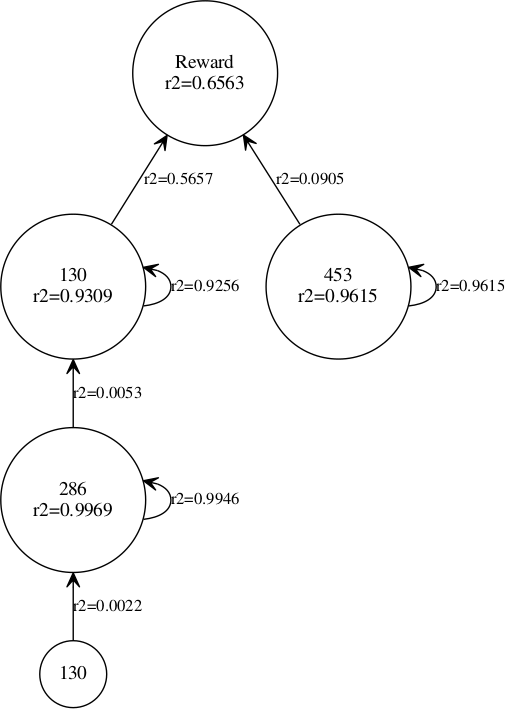
\includegraphics[width=0.4\textwidth]{pictures/experiments/rfs_tree_breakout}
    \centering
    \caption[RFS dependency tree in Breakout]{RFS dependency tree in Breakout.
	    Note how the procedure in this case is not able to correctly 
	    understand the dynamics of the environment and only keeps four 
	    state features without even keeping the action, indicating that in 
	    this case the features extracted by the AE are not suitable for 
	    control-oriented selection.}
    \label{f:rfs_tree_breakout}
\end{figure}
%
%
\begin{figure}
    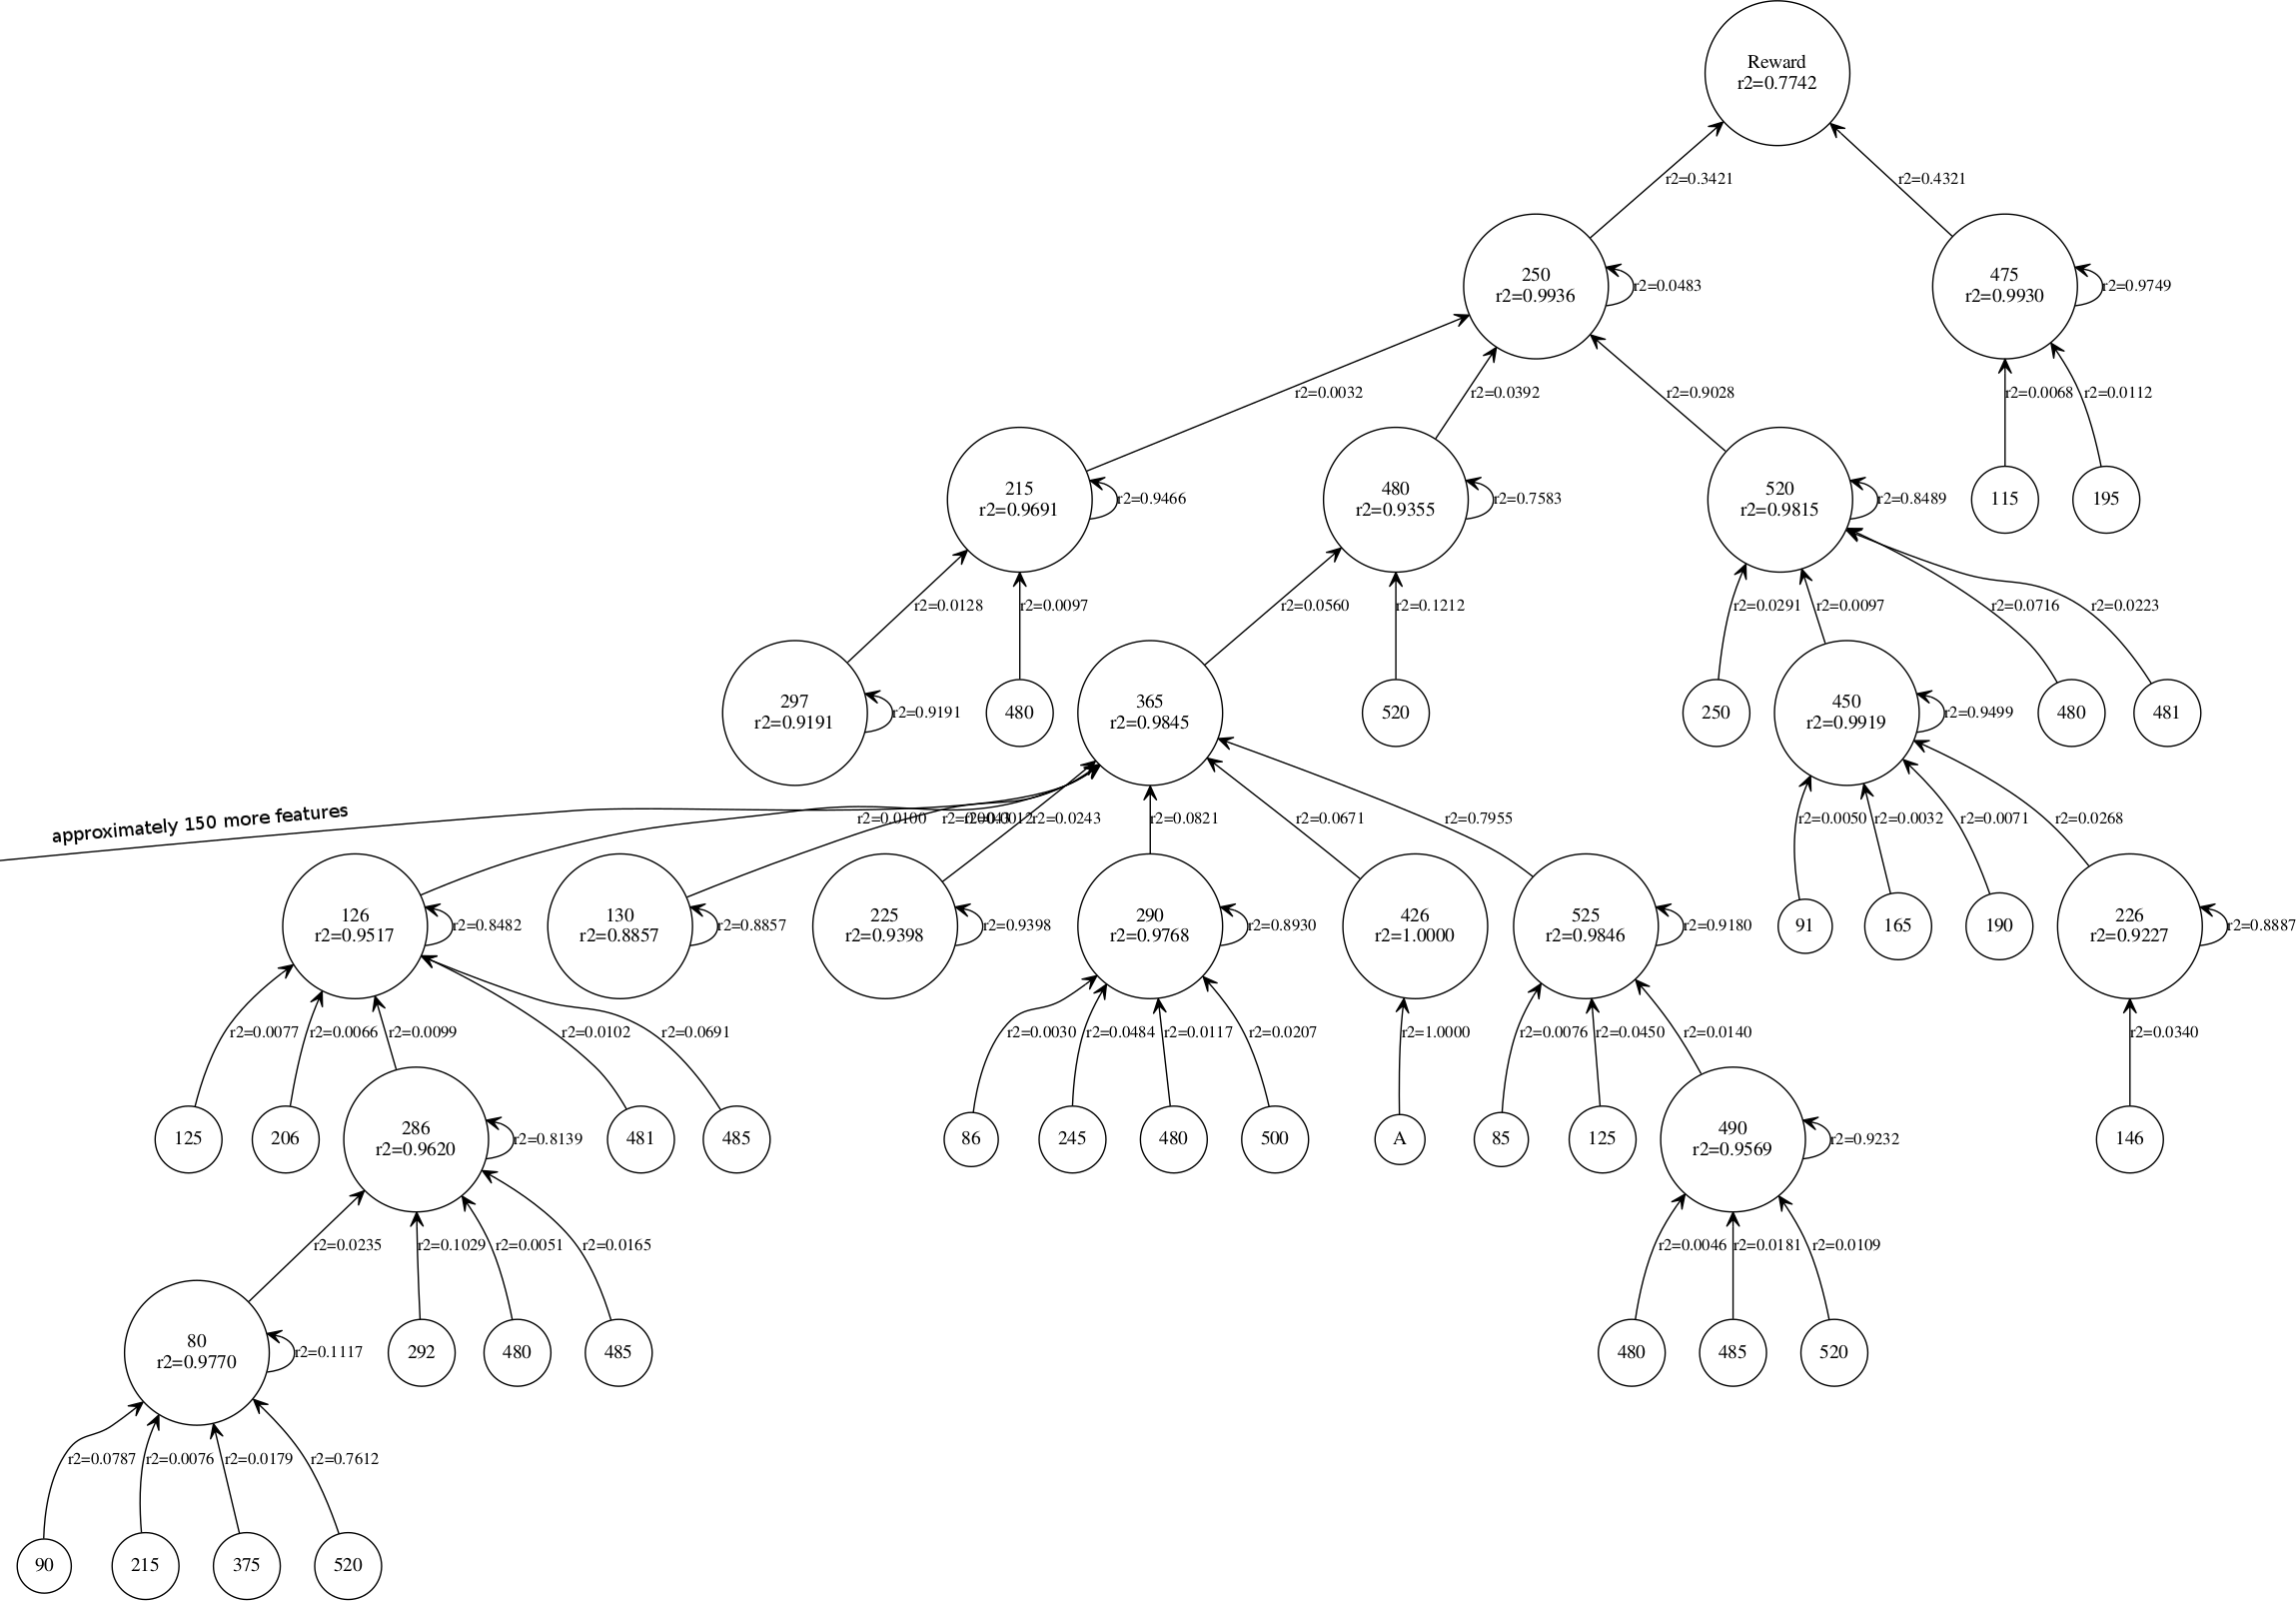
\includegraphics[width=\textwidth]{pictures/experiments/rfs_tree_top_pong}
    \centering
    \caption[RFS dependency tree in Pong]{RFS dependency tree in Pong 
	     (showing only topmost 50 nodes).}
    \label{f:rfs_tree_pong}
\end{figure}
%

\section{Fitted Q-Iteration} \label{s:exp_fqi}
The final part of our experimental methodology consisted in running the full
learning pipeline as described in Algorithm \ref{alg:FQI-DSDF}, and evaluating
the performance of our algorithm in terms of average reward as we did for DQN
and the random policy in Section \ref{s:exp_baseline}. 
As we mentioned in the previous section, due to the excessively long 
computational times of RFS we chose to remove the module entirely from the 
pipeline, resorting to simply keeping those features with nonzero variance 
across the dataset. 
At the same time, we also had to deal with the long runtime for the evaluation 
of the policy during training of FQI (necessary for early stopping), due to a 
general computational complexity of our $Q$ approximation itself, and to an 
internal inefficiency in the software library that we used for Extra-Trees.
We tried to address this issue by training FQI for $50$ iterations at a time
before evaluating the current policy, for a total of $20$ overall evaluations
across $1000$ training iterations. 
This resulted in a noisy evaluation performance, but no more noisy than when we
tested the policy at each iteration. 
We also had to face computational complexity when deciding how many steps
of the main algorithm to run. 
We decided to use a custom $\varphi$ function to reduce $\varepsilon$ (cf.\ 
Section \ref{s:main_alg}) dependent on the total number of steps, so that 
$\varepsilon$ would reach $\varepsilon_{min}$ at the last iteration, and 
at each step would decrease by a fixed quantity as follows:
%
\begin{IEEEeqnarray}{rCl}
    %
    \varphi(\varepsilon) = \varepsilon - \frac{1 - \varepsilon_{min}}{I}
    %
\end{IEEEeqnarray}
%
where $I$ is the total number of iterations (note that the rule only 
applies if $\varepsilon$ is greater that $\varepsilon_{min}$). 
We run a comparison of different values of $\varepsilon$ at 
different steps of the procedure, and we eventually decided to settle for 
running three iterations ($I = 3$) with $\varepsilon_{min} = 0.1$, so that we 
used the values $\varepsilon = 1$, $\varepsilon = 0.55$ and 
$\varepsilon = 0.1$ in sequence. 
This resulted in a tractable runtime for the full algorithm (however 
still in the order of days) and an overall good variety in exploration. 

Moving on to the main results of the FQI training, we report in Tables 
\ref{t:avg_performance_only_ours}, \ref{t:avg_performance_main}, and 
\ref{t:sample_efficiency_main} the performance of our algorithm.
In Table \ref{t:avg_performance_only_ours}, we show the best average evaluation 
score achieved by our agent during the main training procedure.
We note that FQI benefits a great deal by a sufficiently high exploration rate, 
with peak performance typically reached at $\varepsilon\approx0.5$ (this result was often
observed during experiments, even with different configurations for the AE and
FQI). 
Despite being an expected result due to the fact that FQI needs to learn at
once both the value of good and poor states, unlike online neural algorithms 
like DQN that can exploit an intrinsic memory of the architecture to store 
information about previous samples, this also meant that we only reached peak 
performance with our agent at the second main step, with $\varepsilon = 0.55$.
We found that this result was consistent throughout our tests, and we also 
partly attribute to this aspect the inferior performance of our methodology with
respect to the state of the art, because we could never properly exploit the 
learned knowledge to explore the environment to the required degree.
Our agent could consistently achieve a non-trivial performance on all
environments nonetheless, as reported in Table \ref{t:avg_performance_main}, 
reaching on average $25\%$ of DQN's score.

However, despite these poor general results we were able to achieve our main
objective of sample efficiency.
Our agent was consistently able to outperform DQN when considering the amount of
samples collected by our procedure to reach its best performance. 
In Table \ref{t:sample_efficiency_main}, we show how the performance of our 
algorithm at its best is on average almost eight times better than DQN after 
collecting the same amount of samples (roughly $100000$).
At the same time, even if our best scores amounted to at best $40\%$ of DQN's 
score, we were able to achieve them with as little as $0.2\%$ of the collected 
samples (cf.\ Table \ref{t:sample_efficiency_main}).

%
\begin{table}
    \centering
    \begin{tabular}{l c c c c} 
	\hline
	Environment    & Score    & Step       & $\varepsilon$ & FQI epoch  \\ 
	\hline 
	Breakout       & $17$     & $2$ of $3$ & $0.55$        & $400$     \\
	Pong           & $-9$     & $2$ of $3$ & $0.55$        & $350$     \\
	Space Invaders & $460$    & $2$ of $3$ & $0.55$        & $450$     \\
	\hline
    \end{tabular}
    \caption[Performance of our algorithm]{Best average performance reached by 
	    our agent on different environments.}
    \label{t:avg_performance_only_ours}
\end{table}
%
%
\begin{table}
    \centering
    \begin{tabular}{l c c c c} 
	\hline
	Environment    & Random   & Our best & Best DQN      & Score ratio (ours v.\ DQN) \\ 
	\hline 
	Breakout       & $1$      & $17$     & \textbf{319}  & $0.05$                     \\
	Pong           & $-20$    & $-9$     & \textbf{19}   & $0.3$                      \\
	Space Invaders & $174$    & $460$    & \textbf{1125} & $0.4$                      \\
	\hline
    \end{tabular}
    \caption[Performance of our algorithm w.r.t. the baselines]{Best average 
	     performance of our algorithm compared to the baseline algorithms.
	     Note that the score in Pong is shifted to a $[0, 42]$ range to 
	     compute the score ratio.}
    \label{t:avg_performance_main}
\end{table}
%
%
\begin{table}
    \centering
    \begin{tabular}{l c c c c c} 
	\hline
	Environment    & Samples  & Our best      & DQN    & Sample ratio   & Score ratio \\
	\hline 
	Breakout       & $100000$ & \textbf{17}   & $2$    & $0.005$        & $8.5$\\
	Pong           & $100000$ & \textbf{-9}   & $-20$  & $0.002$        & $12$\\
	Space Invaders & $100000$ & \textbf{460}  & $145 $ & $0.003$        & $3.17$\\
	\hline
    \end{tabular}
    \caption[Sample efficiency of our algorithm]{Best average performance 
	    reached by our algorithm compared with the best average performance
	    of DQN using the same number of collected samples. 
	    Sample ratio is computed using the number of samples required by DQN
	    to reach its best performance as reported in Table \ref{t:envs_used}.
	    Note that the score in Pong is shifted to a $[0, 42]$ range to 
	    compute the score ratio.}
    \label{t:sample_efficiency_main}
\end{table}
%
    




